% 
% (c) Copyright 2016 Tabea Mendez
% 
% This source is free: you can redistribute it and/or modify
% it under the terms of the GNU General Public License as published by
% the Free Software Foundation, either version 3 of the License, or
% (at your option) any later version.
% 
% This source is distributed in the hope that it will be useful,
% but WITHOUT ANY WARRANTY; without even the implied warranty of
% MERCHANTABILITY or FITNESS FOR A PARTICULAR PURPOSE.  See the
% GNU General Public License for more details.
% 
% You should have received a copy of the GNU General Public License
% along with this source.  If not, see <http://www.gnu.org/licenses/>.
%
%%%%%%%%%%%%%%%%%%%%%%%%%%%%%%%%%%%%%%%%%%%%%%%%%%%%%%%%%%%%%%%%%%%%%%%%%%%%%%

\section{Quantisierungsprozess}
	Bei der Quantisierung wird jedem Wert eine fixe Nummer zugeordnet.\\[0.2cm]
	\begin{minipage}{0.55\textwidth}
		\begin{tabular}{llll}
			$\bullet$ & Wertebereich/Range: &$-R/2\dots R/2$ &\\
			&$R/2-Q$ ist der höchste Wert.&&\\[0.2cm]
			$\bullet$ &Anzahl Quantisierungsintervalle: & $L = 2^B$&\\[0.2cm]
			$\bullet$ & Anzahl Bits: & $B$ &\\[0.2cm]
			$\bullet$ & Quantisierungsschritt: & \fcolorbox{CadetRed}{white}{$Q = \dfrac{R}{2^B}$}&\\[0.5cm]
			$\bullet$ & Quantisierungsfehler: & \fcolorbox{CadetRed}{white}{$e(nT) = x_Q(nT)-x(nT)$}& $\quad-Q/2\leq e \leq Q/2$\\[0.2cm]
		\end{tabular}
	\end{minipage}
	\begin{minipage}{0.45\textwidth}
		\vspace*{-2cm}\begin{tikzpicture}[>=latex', scale=1.3]
			\draw[->][line width=0.75](0,-1.3)--(0,1.7)node[above]{$x(t)$};
			\draw[->][line width=0.75](-2.7,0)--(3,0)node[below]{$t$};
			\draw[gray, smooth,samples=100,domain=-2.7:2.7, line width=1] plot (\x,{0.875*sin(\x*180/pi)-0.125}) node[right] {$ $};
			
			\draw[line width=0.5](-2,0.65)--(-2,0.5)--node[fill=white]{\footnotesize$Q$}(-2,0.25)--(-2,0.1);
			\draw[line width=0.5,->](-2,0.7)--(-2,0.5);
			\draw[line width=0.5,->](-2,0.05)--(-2,0.25);
			\foreach \i in {-1,-0.75,-0.5,-0.25,0,0.25,0.5,0.75}
			{
				\draw[line width=0.25, dashed](-2.7,\i)--(2.7,\i);
			}

			\draw[line width=0.5](0.2,-1)--(-0.2,-1)node[below left, xshift=4pt]{\footnotesize -R/2};
			\draw[line width=0.5](0.2,1)--(-0.2,1)node[above left, xshift=4pt]{\footnotesize R/2};

			\draw[line width=0.5,gray](1,{0.875*sin(180/pi)-0.125})--++(-0.2,0.2)node[above,darkgray]{\footnotesize $x(nT)$};
			\draw[line width=0.5,CadetRed](1,0.5)--++(0.2,-0.2)node[right, fill=white, yshift=-2pt]{\footnotesize $x_Q(nT)$};


			\foreach \i in {-27,...,27}
			{
				\draw[CadetRed, line width=1] (\i/10-0.05,{round((0.875*sin(\i/10*180/pi)-0.125)*4)/4})--(\i/10+0.05,{round((0.875*sin(\i/10*180/pi)-0.125)*4)/4})--({(\i+1)/10-0.05},{round((0.875*sin((\i+1)/10*180/pi)-0.125)*4)/4})--({(\i+1)/10+0.05},{round((0.875*sin((\i+1)/10*180/pi)-0.125)*4)/4});
			}
			
		\end{tikzpicture}
	\end{minipage}

	\subsection{Quantisierungsfehler / Quantisierungsrauschen}
		\begin{minipage}{0.6\textwidth}
			Wenn das Signal:\\[-0.35cm]
			\begin{itemize}
			\item Wide-Amplitude (gleichmässig ausgesteuert)\\[-0.35cm]
			\item Wide-Band (Breitbandig)\\[-0.35cm]
			\end{itemize}
			ist kann der Quantisierungsfehler als stationärer, gleichverteilter, mittelwertfreier, weisser Zufallsprozess modelliert werden. Mit diesem Modell wird der Quantisierungsfehler (nicht-linear, deterministisch) zu einem \textbf{linearen und stochasitschen} Modell. 
		\end{minipage}\begin{minipage}{0.05\textwidth}$ $\end{minipage}
		\begin{minipage}{0.5\textwidth}
			\begin{tikzpicture}[>=latex', scale=1.5]
				\draw[line width=1](-1,-0.5)--node[below]{\footnotesize Quantisierer}(1,-0.5)--(1,0.5)--(-1,0.5)--cycle;
				\draw[line width=1](0,0)circle(0.15)node{$+$};
				\draw[line width=1,->](-1.8,0)node[above right]{\footnotesize$x(n)$}--(-0.15,0);
				\draw[line width=1,->](0,0.9)node[below right, yshift=3pt]{\footnotesize$e(n)$}--(0,0.15);
				\draw[line width=1,->](0.15,0)--(1.8,0)node[above left]{\footnotesize$x_Q(n)$};
			\end{tikzpicture} 
		\end{minipage}\\[0.2cm]
		
		\textbf{Eigenschaften des Quanitsierungsrauschens}
		\begin{description}
		 \item [Gleichverteiltes Rauschen:]$ $\\[0cm]
			\begin{minipage}{0.37\textwidth}
				\fcolorbox{CadetRed}{white}{$p(e)=\begin{cases}1/Q, & -Q/2\leq e\leq Q/2\\0, & \text{sonst}\end{cases}$}
			\end{minipage}
			\begin{minipage}{0.27\textwidth}
				\begin{tikzpicture}[>=latex', scale=1.3]
					\draw[->][line width=0.75](0,-0.3)--(0,1.2)node[right]{\footnotesize$p(e)$};
					\draw[->][line width=0.75](-1.5,0)--(1.7,0)node[below]{\footnotesize$e$};
					\draw[line width=1,CadetRed](-1.5,0)--(-1,0)--(-1,0.7)node[left]{\footnotesize$\dfrac{1}{Q}$}--(1,0.7)--(1,0)--(1.5,0);
					\draw[line width=0.5](-1,0.1)--(-1,-0.1)node[below]{\footnotesize -$Q/2$};
					\draw[line width=0.5](1,0.1)--(1,-0.1)node[below]{\footnotesize$Q/2$};
				\end{tikzpicture}
			\end{minipage}
			\begin{minipage}{0.3\textwidth}
				\textbf{Mittelwert:}  $\;\,\mu_e = E[e] = 0$\\[0.1cm]
				\textbf{Varianz:} $\qquad\sigma^2_e = E[e^2] = \dfrac{Q^2}{12}$
			\end{minipage}
		 \item[Weisses Rauschen (Leistungsdichtespektrum und Autokorrelation):]$ $\\[0.2cm]
			\begin{minipage}{0.37\textwidth}
				\fcolorbox{CadetRed}{white}{$S_{ee}(f)=\begin{cases}\dfrac{\sigma^2_e}{f_s}, & -\dfrac{f_s}{2}\leq f\leq \dfrac{f_s}{2}\\0, & \text{sonst}\end{cases}$}
			\end{minipage}
			\begin{minipage}{0.27\textwidth}
				\begin{tikzpicture}[>=latex', scale=1.3]
					\draw[->][line width=0.75](0,-0.3)--(0,1.2)node[right]{\footnotesize$S_{ee}(f)$};
					\draw[->][line width=0.75](-1.5,0)--(1.7,0)node[below]{\footnotesize$f$};
					\draw[line width=1,CadetRed](-1.5,0)--(-1,0)--(-1,0.7)node[left]{\footnotesize$\dfrac{\sigma_e^2}{f_s}$}--(1,0.7)--(1,0)--(1.5,0);
					\draw[line width=0.5](-1,0.1)--(-1,-0.1)node[below]{\footnotesize -$f_s/2$};
					\draw[line width=0.5](1,0.1)--(1,-0.1)node[below]{\footnotesize$f_s/2$};

					\draw[CadetRed, line width=0.5, fill](1.3,0.3)circle(0.03);
					\draw[CadetRed, line width=0.5, fill](1.45,0.3)circle(0.03);
					\draw[CadetRed, line width=0.5, fill](1.6,0.3)circle(0.03);
					\draw[CadetRed, line width=0.5, fill](-1.3,0.3)circle(0.03);
					\draw[CadetRed, line width=0.5, fill](-1.45,0.3)circle(0.03);
					\draw[CadetRed, line width=0.5, fill](-1.6,0.3)circle(0.03);
				\end{tikzpicture}
			\end{minipage}
			\begin{minipage}{0.3\textwidth}
				\begin{tikzpicture}[>=latex', scale=1.3]
					\draw[->][line width=0.75](0,-0.3)--(0,1.2)node[right]{\footnotesize$R_{ee}(k)$};
					\draw[->][line width=0.75](-0.5,0)--(0.7,0)node[below]{\footnotesize$k$};
					\draw[->,line width=1,CadetRed](0,0)--(0,0.8)node[left]{\footnotesize$\sigma_e^2\delta(k)$};
					\draw[line width=0.5,white](-0.8,0.1)--(-0.8,-0.1)node[below right]{\footnotesize$f_s/2$};

				\end{tikzpicture}
			\end{minipage}
		 \item[Unkorreliert mit dem Signal \bm{$x(n)$}:] $R_{ex} = E[e(n+k)\cdot x(n)] = 0$
		 \item[Signal-Rausch-Abstand (SNR):]$ $\\[0.2cm]
			\begin{minipage}{0.4\textwidth}
				Rauschleistung:\\[0.2cm]
				$P_N = E[e^2] =  \dfrac{1}{Q}\myint{-Q/2}{Q/2}{e^2}{e} = \dfrac{Q^2}{12}$
			\end{minipage}
			\begin{minipage}{0.5\textwidth}
				Signalleistung (voll ausgesteuert und gleichverteilt):\\[0.2cm]
				$P_S = E[s^2] = \dfrac{1}{R}\myint{-R/2}{R/2}{s^2}{s} = \dfrac{R^2}{12}$
			\end{minipage}\\[0.2cm]
			$\text{SNR} = 10\log_{10}\left(\dfrac{P_S}{P_N}\right) = 10\log_{10}\left(\dfrac{R^2/12}{Q^2/12}\right) = 20\log_{10}\left(\dfrac{R}{Q}\right) = 20\log_{10}\left(2^B\right) = B\cdot 6\db$\\[0.2cm]
			Pro Bit wird SNR um Faktor 4 besser.\\[0.2cm]
			\fcolorbox{CadetRed}{white}{$\text{SNR} = B\cdot 6\db$}$\quad$

			
		\end{description}
\newpage
\section{Oversampling $\Leftrightarrow$ Quantisierungsstufen}
	Die Idee von Oversampling ist, durch schnelleres Abstasten des Signals, weniger Bits für den Quanitsierer spendieren zu müssen aber dennoch die selbe Quantisierungsqualität beizubehalten.\\[0.2cm]
	\fcolorbox{CadetRed}{white}{schneller Abtasten + weniger Quantisierungsintervalle = gleiche Quanitsierungsqualität}\\[0.2cm]
	\fcolorbox{CadetRed}{white}{schneller Abtasten + gleich viele Quantisierungsintervalle = bessere Quanitsierungsqualität}\\[-0.2cm]
	
	\subsection{Vergleich der zwei unterschiedlich schnell abgetasteten Systeme}
	\begin{tabular}{|l|c|c|}
	\hline
	& $\qquad\qquad\qquad\qquad\qquad\qquad\qquad$&$\qquad\qquad\qquad\qquad\qquad\qquad\qquad$\\[-0.4cm]
		&langsame Abtastfrequenz $f_s$ & schnelle Abtastfrequenz $f'_s$\\
		&viele Bits pro Sample $B$ & wenig Bits pro Sample $B'$\\[0.1cm]
	\hline&\multicolumn{2}{c|}{}\\[-0.3cm]
		Oversamplingrate: & \multicolumn{2}{c|}{\fcolorbox{CadetRed}{white}{$L = \dfrac{f'_s}{f_s}$}}\\[0.45cm]
	\hline&&\\[-0.3cm]
		Quantisierungsintervall: & $Q = \dfrac{R}{2^{B}}$&$Q' = \dfrac{R}{2^{B'}}$\\[0.25cm]
	\hline&&\\[-0.3cm]
		Rauschleistung: & $\sigma_e^2 = \dfrac{Q^2}{12}$& $\sigma_e'^2 = \dfrac{Q'^2}{12}$\\[0.25cm]
	\hline&\multicolumn{2}{c|}{}\\[-0.3cm]
		Leistungsdichtespektrum: &\multicolumn{2}{c|}{\fcolorbox{CadetRed}{white}{$\dfrac{\sigma_e^2}{f_s} = \dfrac{\sigma_e'^2}{f'_s}\qquad\Rightarrow\qquad \sigma_e^2 = \dfrac{\sigma_e'^2}{L}$}}\\[0.5cm]
	\hline&\multicolumn{2}{c|}{}\\[-0.3cm]
		Bitgewinn: & \multicolumn{2}{c|}{$L = \dfrac{\sigma_e'^2}{\sigma_e^2} = \dfrac{Q'^2}{Q^2} = 2^{2(B-B')} = 2^{2\Delta B}$}\\[0.45cm]
		1 Bit $\mathrel{\hat=}$ 4 $\times$ schneller abtasten & \multicolumn{2}{c|}{\fcolorbox{CadetRed}{white}{$\Delta B = 0.5\cdot \log_2(L)$}}\\[0.25cm]
	\hline
	\end{tabular}\\
% 	\begin{center}
		\begin{tikzpicture}[>=latex', scale=1.7]
			\draw[->][line width=0.75](0,-0.3)--(0,1.2)node[right]{\footnotesize$S_{ee}(f)$};
			\draw[->][line width=0.75](-2.5,0)--(2.7,0)node[below]{\footnotesize$f$};
			\draw[line width=1,CadetRed](-2.5,0)--(-2,0)--(-2,0.7)node[left]{\footnotesize$\dfrac{\sigma_e'^2}{f'_s}$}--(2,0.7)--(2,0)--(2.5,0);
			\draw[line width=0.5](-2,0.1)--(-2,-0.1)node[below=-1pt]{\footnotesize -$\dfrac{f'_s}{2}$};
			\draw[line width=0.5](2,0.1)--(2,-0.1)node[below=-1pt]{\footnotesize $\dfrac{f'_s}{2}$};

			\draw[line width=0.01,gray,fill, opacity=0.5](-0.7,0)--(-0.7,0.7)--(0.7,0.7)--(0.7,0)--cyclenode at (0.25,0.4)[darkgray, opacity=1]{$\sigma_e^2$};

			\draw[line width=1,blueT](-2,0)--(-0.7,0)--(-0.7,0.7)node[above]{\footnotesize$\dfrac{\sigma_e^2}{f_s}$}--(0.7,0.7)--(0.7,0)--(2,0);
			\draw[line width=0.5](-0.7,0.1)--(-0.7,-0.1)node[below]{\footnotesize -$\dfrac{f_s}{2}$};
			\draw[line width=0.5](0.7,0.1)--(0.7,-0.1)node[below]{\footnotesize $\dfrac{f_s}{2}$};

			\draw[CadetRed, line width=0.5, fill](2.3,0.3)circle(0.03);
			\draw[CadetRed, line width=0.5, fill](2.45,0.3)circle(0.03);
			\draw[CadetRed, line width=0.5, fill](2.6,0.3)circle(0.03);
			\draw[CadetRed, line width=0.5, fill](-2.3,0.3)circle(0.03);
			\draw[CadetRed, line width=0.5, fill](-2.45,0.3)circle(0.03);
			\draw[CadetRed, line width=0.5, fill](-2.6,0.3)circle(0.03);
		\end{tikzpicture}
% 	\end{center}

\section{Noise Shaping}\label{NoiseShapingHerleitung}$ $\\[-2.2cm]
	\begin{minipage}{0.65\textwidth}
		Die Idee von Noise Shaping ist, das Quantisierungsrauschen so umzuverteilen, dass im Frequenzband des langsam abgetasteten Systems möglichst wenig Rauschleistung vorhanden ist. Das Quantisierungsrauschen wird also im Prinzip zuerst gefiltert.\\[-2.3cm]
	\end{minipage}
	\begin{minipage}{0.05\textwidth} $ $\end{minipage}
	\begin{minipage}{0.35\textwidth}
		\begin{tikzpicture}[>=latex', scale=1.5]
			\draw[line width=1](-1,-0.5)--node[below]{\footnotesize Quantisierer}(1,-0.5)--(1,1.25)--(-1,1.25)--cycle;
			\draw[line width=1](-0.5,0.5)--node[above=1.5pt]{\footnotesize $H_{NS}(f)$}(0.5,0.5)--(0.5,1.)--(-0.5,1.)--cycle;
			\draw[line width=1](0,0)circle(0.15)node{$+$};
			\draw[line width=1,->](-1.8,0)node[above right]{\footnotesize$x(n)$}--(-0.15,0);
			\draw[line width=1,->](0,1.65)node[below right, yshift=3pt]{\footnotesize$e(n)$}--(0,1);
			\draw[line width=1,->](0,0.5)node[below right]{\footnotesize$\varepsilon(n)$}--(0,0.15);
			\draw[line width=1,->](0.15,0)--(1.8,0)node[above left]{\footnotesize$x_Q(n)$};
		\end{tikzpicture}
	\end{minipage}\\[0.2cm]
	\fcolorbox{CadetRed}{white}{$\sigma_e^2 = \dfrac{\sigma_e'^2}{f'_s}\myint{-f_s/2}{f_s/2}{|H_{NS}(f)|^2}{f}$}$\qquad$\fcolorbox{CadetRed}{white}{$|H_{NS}(f)|^2 = \left|2\,\sin\left(\dfrac{\pi f}{f_s'}\right)\right|^{2p}\quad$ für $-\dfrac{f_s'}{2}\leq f\leq \dfrac{f_s'}{2}$}\\[0.2cm]
	
	$\sigma_e^2\;\; \stackrel{\mathrm{|f|<<f_s'/2}}\approx \;\;\dfrac{\sigma_e'^2}{f'_s}\myint{-f_s/2}{f_s/2}{\left(\dfrac{2\pi f}{f_s'}\right)^{2p}}{f} = \sigma_e'^2\,\dfrac{\pi^{2p}}{2p+1}\,\dfrac{1}{L^{2p+1}}\qquad \Rightarrow\qquad \dfrac{\sigma_e^2}{\sigma_e'^2} = 2^{-2(B-B')} = 2^{-2\Delta B} = \dfrac{\pi^{2p}}{2p+1}\,\dfrac{1}{L^{2p+1}}$\\[0.2cm]
	\begin{minipage}{0.55\textwidth}
		\begin{tikzpicture}[>=latex', scale=1.7]
			\draw[->][line width=0.75](0,-0.3)--(0,1.2)node[above]{\footnotesize$S_{ee}(f)$ / $S_{\varepsilon\varepsilon}(f)$};
			\draw[->][line width=0.75](-2.5,0)--(2.7,0)node[below]{\footnotesize$f$};
			\draw[line width=1,CadetRed](-2.5,0)--(-2,0)--(-2,0.7)node[left]{\footnotesize$\dfrac{\sigma_e'^2}{f'_s}$}--(2,0.7)--(2,0)--(2.5,0);
			\draw[line width=0.5](-2,0.1)--(-2,-0.1)node[below=-1pt]{\footnotesize -$\dfrac{f'_s}{2}$};
			\draw[line width=0.5](2,0.1)--(2,-0.1)node[below=-1pt]{\footnotesize $\dfrac{f'_s}{2}$};

			\draw[line width=0.01,gray,fill, opacity=0.5](-0.7,0)--(-0.7,0.7)--(0.7,0.7)--(0.7,0)--cyclenode at (0.25,0.4)[darkgray, opacity=1]{$ $};

			\draw[line width=1,blueT](-2,0)--(-0.7,0)--(-0.7,0.7)node[above]{\footnotesize$\dfrac{\sigma_e^2}{f_s}$}--(0.7,0.7)--(0.7,0)--(2,0);
			\draw[line width=0.5](-0.7,0.1)--(-0.7,-0.1)node[below]{\footnotesize -$\dfrac{f_s}{2}$};
			\draw[line width=0.5](0.7,0.1)--(0.7,-0.1)node[below]{\footnotesize $\dfrac{f_s}{2}$};

			\draw[CadetRed, line width=0.5, fill](2.3,0.3)circle(0.03);
			\draw[CadetRed, line width=0.5, fill](2.45,0.3)circle(0.03);
			\draw[CadetRed, line width=0.5, fill](2.6,0.3)circle(0.03);
			\draw[CadetRed, line width=0.5, fill](-2.3,0.3)circle(0.03);
			\draw[CadetRed, line width=0.5, fill](-2.45,0.3)circle(0.03);
			\draw[CadetRed, line width=0.5, fill](-2.6,0.3)circle(0.03);

			\draw[black, smooth,samples=100,domain=-2:2, line width=1](-2,0.7)--plot (\x,{0.25*abs(2*sin(\x*pi/4.5*180/pi))^2})node[above] {\footnotesize$\dfrac{\sigma_e'^2}{f_s'}|H_{NS}(f)|^2$}--(2,0.7);
			\draw[black, smooth,samples=100,domain=-0.7:0.7, line width=1, fill, opacity=0.5](-0.7,0)--plot (\x,{0.25*abs(2*sin(\x*pi/4.5*180/pi))^2}) node[right] {$ $}--(0.7,0);
		\end{tikzpicture}
	\end{minipage}
	\begin{minipage}{0.48\textwidth}
		\fcolorbox{CadetRed}{white}{$\Delta B = (p+0.5)\,\log_2(L)-0.5\,\log_2\left(\dfrac{\pi^{2p}}{2p+1}\right)$}
	\end{minipage}
% 	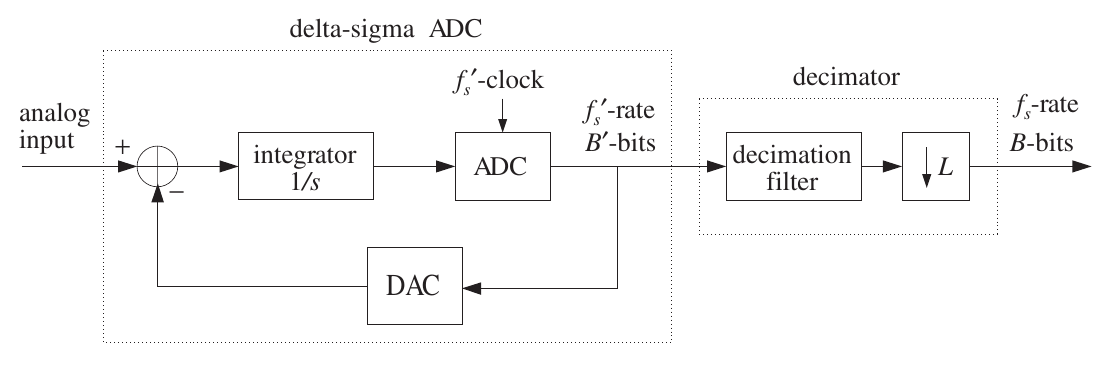
\includegraphics[width = 0.6\textwidth]{pic/deltaSigma.png}\centering
\newpage
\section{Digital-Analog-Wandler}
	\begin{minipage}{0.55\textwidth}
		Es gibt verschiedene Arten um Bitmuster in einen analogen Wert zu wandeln.
		\begin{itemize}
		 \item Unipolar Natural Binary
		 \item Bipolar Offset Binary
		 \item Bipolar Two's Complement
		\end{itemize}
	\end{minipage}\begin{minipage}{0.05\textwidth} $ $\end{minipage}
	\begin{minipage}{0.5\textwidth}
		\begin{tikzpicture}[>=latex', scale=1.5]
			\draw[line width=1](-0.5,-0.75)--(0.5,-0.75)--(0.5,0.75)--(-0.5,0.75)--cycle;
			\node at(0,0){\footnotesize DAC};
			\draw[line width=1,->](0.5,0)--node[above]{\footnotesize$x_Q$}node[below]{\footnotesize \parbox{1cm}{\centering analog\\ output}}(1.5,0);
			\draw[line width=1,->](-1.5,0.5)node[left]{\footnotesize $b_1$}--node[above]{\footnotesize MSB}(-0.5,0.5);
			\draw[line width=1,->](-1.5,0.25)node[left]{\footnotesize $b_2$}--node[above]{\footnotesize }(-0.5,0.25);
			\draw[line width=1,->](-1.5,0)node[left]{\footnotesize $b_3$}--node[above]{\footnotesize }(-0.5,-0);
			\node[rotate=90] at (-1,-0.25){\footnotesize $\cdots$};
			\draw[line width=1,->](-1.5,-0.5)node[left]{\footnotesize $b_B$}--node[below]{\footnotesize LSB}(-0.5,-0.5);
			\node[rotate=90] at (-2.1,-0){\footnotesize $B$ input bits};

			\draw[line width=1,fill](0,-0.75)--(-0,-1)circle(0.05)node[right=2pt]{\footnotesize R \tiny (Reference)};
		\end{tikzpicture} 
	\end{minipage}

	\begin{tabularx}{1.0025\textwidth}{|p{5.5cm}|p{5.5cm}|p{6cm}|}
	 \hline&&\\[-0.35cm]
		\textbf{Unipolar Natural Binary} & \textbf{Bipolar Offset Binary} & \textbf{Bipolar Two's Complement}\\[0.1cm]
	 \hline&&\\[-0.35cm]
		\begin{tikzpicture}[>=latex', scale=1.7]
			\draw[->][line width=0.75](0,-0.1)--(0,2.2)node[above]{\footnotesize$x_Q$};
			\draw[->][line width=0.75](-0.1,0)--(2,0)node[right]{\footnotesize$B$};
			\draw[line width=0.5](0/4,0.1)--(0/4,-0.1)node[below]{\tiny $000$};
			\draw[line width=0.5](0.1,0/4)--(-0.1,0/4)node[left]{\tiny $0$};

			\draw[line width=1,CadetRed,dashed](0,0)--(2,2);
			\foreach \i in {0,...,7}
			{
				\draw[line width=0.5, gray,dashed](0,\i/4)--(\i/4,\i/4);
				\draw[line width=0.5, gray,dashed](\i/4,0)--(\i/4,\i/4);
				\draw[line width=1,CadetRed,fill](\i/4,\i/4)circle(0.05);
			}

			\draw[line width=0.5](1/4,0.1)--(1/4,-0.1)node[below, yshift=-5pt]{\tiny $001$};
			\draw[line width=0.5](2/4,0.1)--(2/4,-0.1)node[below]{\tiny $010$};
			\draw[line width=0.5](3/4,0.1)--(3/4,-0.1)node[below, yshift=-5pt]{\tiny $011$};
			\draw[line width=0.5](4/4,0.1)--(4/4,-0.1)node[below]{\tiny $100$};
			\draw[line width=0.5](5/4,0.1)--(5/4,-0.1)node[below, yshift=-5pt]{\tiny $101$};
			\draw[line width=0.5](6/4,0.1)--(6/4,-0.1)node[below]{\tiny $110$};
			\draw[line width=0.5](7/4,0.1)--(7/4,-0.1)node[below, yshift=-5pt]{\tiny $111$};

			\draw[line width=0.5](0.1,8/4)--(-0.1,8/4)node[left]{\tiny $R$};
			\draw[line width=0.5](0.1,7/4)--(-0.1,7/4)node[left]{\tiny $7Q$};
			\draw[line width=0.5](0.1,6/4)--(-0.1,6/4)node[left]{\tiny $6Q$};
			\draw[line width=0.5](0.1,5/4)--(-0.1,5/4)node[left]{\tiny $5Q$};
			\draw[line width=0.5](0.1,4/4)--(-0.1,4/4)node[left]{\tiny $4Q$};
			\draw[line width=0.5](0.1,3/4)--(-0.1,3/4)node[left]{\tiny $3Q$};
			\draw[line width=0.5](0.1,2/4)--(-0.1,2/4)node[left]{\tiny $2Q$};
			\draw[line width=0.5](0.1,1/4)--(-0.1,1/4)node[left]{\tiny $Q$};
		\end{tikzpicture}&
		\begin{tikzpicture}[>=latex', scale=1.7]
			\draw[->][line width=0.75](0,-0.1)--(0,2.2)node[above]{\footnotesize$x_Q$};
			\draw[->][line width=0.75](-0.1,1)--(2,1)node[right]{\footnotesize$B$};

			\draw[line width=0.5](4/4,1.1)--(4/4,0.9)node[below]{\tiny $100$};
			\draw[line width=0.5](0.1,0/4)--(-0.1,0/4)node[left]{\tiny $-R/2$};

			\draw[line width=1,CadetRed,dashed](0,0)--(2,2);
			\foreach \i in {1,...,3,5,6,7}
			{
				\draw[line width=0.5, gray,dashed](0,\i/4)--(\i/4,\i/4);
			}
			\foreach \i in {1,...,7}
			{
				\draw[line width=0.5, gray,dashed](\i/4,1)--(\i/4,\i/4);
			}
			\foreach \i in {0,...,7}
			{
				\draw[line width=1,CadetRed,fill](\i/4,\i/4)circle(0.05);
			}

			\draw[line width=0.5](1/4,0.9)--(1/4,1.1)node[above, fill=white]{\tiny $001$};
			\draw[line width=0.5](3/4,0.9)--(3/4,1.1)node[above, fill=white]{\tiny $011$};
			\draw[line width=0.5](2/4,0.9)--(2/4,1.1)node[above,yshift=5pt]{\tiny $010$};
			\draw[line width=0.5](5/4,1.1)--(5/4,0.9)node[below, yshift=-5pt]{\tiny $101$};
			\draw[line width=0.5](6/4,1.1)--(6/4,0.9)node[below]{\tiny $110$};
			\draw[line width=0.5](7/4,1.1)--(7/4,0.9)node[below, yshift=-5pt]{\tiny $111$};

			\draw[line width=0.5](0.1,8/4)--(-0.1,8/4)node[left]{\tiny $R/2$};
			\draw[line width=0.5](0.1,7/4)--(-0.1,7/4)node[left]{\tiny $3Q$};
			\draw[line width=0.5](0.1,6/4)--(-0.1,6/4)node[left]{\tiny $2Q$};
			\draw[line width=0.5](0.1,5/4)--(-0.1,5/4)node[left]{\tiny $Q$};
			\draw[line width=0.5](0.1,4/4)--(-0.1,4/4)node[left]{\tiny $0$};
			\draw[line width=0.5](0.1,3/4)--(-0.1,3/4)node[left]{\tiny $-Q$};
			\draw[line width=0.5](0.1,2/4)--(-0.1,2/4)node[left]{\tiny $-2Q$};
			\draw[line width=0.5](0.1,1/4)--(-0.1,1/4)node[left]{\tiny $-3Q$};
		\end{tikzpicture}&
		\begin{tikzpicture}[>=latex', scale=1.7]
			\draw[->][line width=0.75](0,-1.2)--(0,1.2)node[above]{\footnotesize$x_Q$};
			\draw[->][line width=0.75](-0.1,0)--(2,0)node[right]{\footnotesize$B$};

			\draw[line width=0.5](0/4,0.1)--(0/4,-0.1)node[below]{\tiny $ $};
			\draw[line width=0.5](0.1,0/4)--(-0.1,0/4)node[left]{\tiny $0$};

			\draw[line width=1,CadetRed,dashed](0,0)--(1,1);
			\foreach \i in {0,...,3}
			{
				\draw[line width=0.5, gray,dashed](0,\i/4)--(\i/4,\i/4);
				\draw[line width=0.5, gray,dashed](\i/4,0)--(\i/4,\i/4);
				\draw[line width=1,CadetRed,fill](\i/4,\i/4)circle(0.05);
			}

			\draw[line width=1,CadetRed,dashed](1,-1)--(2,0);
			\foreach \i in {4,...,7}
			{
				\draw[line width=0.5, gray,dashed](0,-2+\i/4)--(\i/4,-2+\i/4);
				\draw[line width=0.5, gray,dashed](\i/4,0)--(\i/4,-2+\i/4);
				\draw[line width=1,CadetRed,fill](\i/4,-2+\i/4)circle(0.05);
			}

			\draw[line width=0.5](2/4,0.1)--(2/4,-0.1)node[below,fill=white]{\tiny $010$};
			\draw[line width=0.5](1/4,0.1)--(1/4,-0.1)node[below, yshift=-5pt]{\tiny $001$};
			\draw[line width=0.5](3/4,0.1)--(3/4,-0.1)node[below, yshift=-5pt]{\tiny $011$};
			\draw[line width=0.5](4/4,-0.1)--(4/4,0.1)node[above]{\tiny $100$};
			\draw[line width=0.5](5/4,-0.1)--(5/4,0.1)node[above, yshift=5pt]{\tiny $101$};
			\draw[line width=0.5](6/4,-0.1)--(6/4,0.1)node[above]{\tiny $110$};
			\draw[line width=0.5](7/4,-0.1)--(7/4,0.1)node[above, yshift=5pt]{\tiny $111$};

			\draw[line width=0.5](0.1,-4/4)--(-0.1,-4/4)node[left]{\tiny $R/2$};
			\draw[line width=0.5](0.1,-3/4)--(-0.1,-3/4)node[left]{\tiny $-3Q$};
			\draw[line width=0.5](0.1,-2/4)--(-0.1,-2/4)node[left]{\tiny $-2Q$};
			\draw[line width=0.5](0.1,-1/4)--(-0.1,-1/4)node[left]{\tiny $-Q$};
			\draw[line width=0.5](0.1,4/4)--(-0.1,4/4)node[left]{\tiny $R/2$};
			\draw[line width=0.5](0.1,3/4)--(-0.1,3/4)node[left]{\tiny $3Q$};
			\draw[line width=0.5](0.1,2/4)--(-0.1,2/4)node[left]{\tiny $2Q$};
			\draw[line width=0.5](0.1,1/4)--(-0.1,1/4)node[left]{\tiny $Q$};
		\end{tikzpicture}\\[0.1cm]
	 \hline&&\\[-0.35cm]
		\fcolorbox{CadetRed}{white}{$x_Q = R\,\mysum{n=1}{B}{b_n\,2^{-n}}$}&\fcolorbox{CadetRed}{white}{$x_Q = R\,\left(\mysum{n=1}{B}{b_n\,2^{-n}}-\dfrac{1}{2}\right)$}&\fcolorbox{CadetRed}{white}{$x_Q = R\, \left(\overline{b_1}\,2^{-1}+\mysum{n=2}{B}{b_n\,2^{-n}}-\dfrac{1}{2}\right)$}\\[0.5cm]
	 \hline&&\\[-0.35cm]
		\fcolorbox{CadetRed}{white}{$x_Q = Q\cdot m$}$\quad$\fcolorbox{CadetRed}{white}{$m = \mysum{n=1}{B}{b_n\,2^{B-n}}$} & \fcolorbox{CadetRed}{white}{$x_Q = Q\cdot m'$}$\quad$\fcolorbox{CadetRed}{white}{$m' = m - 2^{B-1}$} & \fcolorbox{CadetRed}{white}{$x_Q = Q\cdot m''$}$\quad$\newline\fcolorbox{CadetRed}{white}{$m'' = m + (($-$1)^{b_1}-1)\,2^{B-1}$} \\[0.5cm]
	 \hline&&\\[-0.35cm]
		$m = 0,1,2,...,2^{B}-1$ & $m' = $-$2^{B-1},...,$-$1,0,1,...,2^{B-1}-1$& $m'' = $-$2^{B-1},...,$-$1,0,1,...,2^{B-1}-1$\\[0.1cm]
	 \hline&&\\[-0.35cm]
		$x_{Qmin} = 0$ & $x_{Qmin} = -R/2 $ &$x_{Qmin} = -R/2$ \\[0.1cm]
	\hline&&\\[-0.35cm]
		$x_{Qmax} = R-Q$ & $x_{Qmax} = R/2-Q$ &$x_{Qmax} = R/2-Q$ \\[0.1cm]
	 \hline	 
	\end{tabularx}\\

\section{Analog-Digital-Wandler}
	\vspace*{-0.3cm}\begin{minipage}{0.32\textwidth}
		Ein Analog-Digital-Wandler quantisiert einen analogen Wert in ein digitales Bitmuster.\\
	\end{minipage}\begin{minipage}{0.05\textwidth}$ $\end{minipage}
	\begin{minipage}{0.4\textwidth}
		\begin{tikzpicture}[>=latex', scale=1.5]
			\draw[line width=1](-0.5,-0.75)--(0.5,-0.75)--(0.5,0.75)--(-0.5,0.75)--cycle;
			\node at(0,0){\footnotesize ADC};
			\draw[line width=1,->](-1.5,0)--node[above]{\footnotesize$x$}node[below]{\footnotesize \parbox{1cm}{\centering analog\\ input}}(-0.5,0);
			\draw[line width=1,->](0.5,0.5)--node[above]{\footnotesize MSB}(1.5,0.5)node[right]{\footnotesize $b_1$};
			\draw[line width=1,->](0.5,0.25)--node[above]{\footnotesize }(1.5,0.25)node[right]{\footnotesize $b_2$};
			\draw[line width=1,->](0.5,0)--node[above]{\footnotesize }(1.5,-0)node[right]{\footnotesize $b_3$};
			\node[rotate=90] at (1,-0.25){\footnotesize $\cdots$};
			\draw[line width=1,->](0.5,-0.5)--node[below]{\footnotesize LSB}(1.5,-0.5)node[right]{\footnotesize $b_B$};
			\node[rotate=90] at (2.1,-0){\footnotesize $B$ output bits};

			\draw[line width=1,fill](0,-0.75)--(-0,-1)circle(0.05)node[right=2pt]{\footnotesize R \tiny (Reference)};
		\end{tikzpicture}
	\end{minipage}

	\begin{minipage}[t]{0.66\textwidth}
		\textbf{Successive Approximation:}\\[0.2cm]
		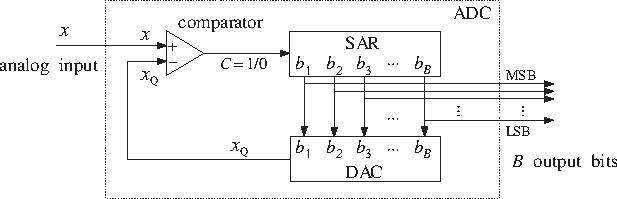
\includegraphics[width = 0.8\textwidth]{pic/sar.pdf}\\[0.2cm]
		Weil der SAR-AD-Wandler immer abrundet, muss vor dem Quantisieren zum Eingangswert eine halber Quantisierungsschritt dazugezählt werden\\[0.2cm]
		\fcolorbox{CadetRed}{white}{$y = x + \dfrac{1}{2}Q$}
	\end{minipage}
	\begin{minipage}[t]{0.3\textwidth}
		\begin{enumerate}
		\item Alle bits auf null setzen
		\item $b_1$ auf 1 setzen\\
			$x_Q>x\quad\rightarrow\quad b_1 = 0$\\
			$x_Q<x\quad\rightarrow\quad b_1 = 1$
		\item $b_2$ auf 1 setzen\\
			$x_Q>x\quad\rightarrow\quad b_2 = 0$\\
			$x_Q<x\quad\rightarrow\quad b_2 = 1$
		\item mit allen Bits wiederholen
		\item $b_B$ auf 1 setzen\\
			$x_Q>x\quad\rightarrow\quad b_B = 0$\\
			$x_Q<x\quad\rightarrow\quad b_B = 1$
		\end{enumerate}	
	\end{minipage}

\section{Dither}
	Dither ist ein kleines weisses Rauschen, dass vor dem Quantisieren zum Signal addiert wird.\\ Dies wird gemacht um:
	\begin{itemize}
	 \item Quantisierungsverzerrungen (Muster) zu eliminieren 
	 \item Das Quantisierungsrauschen weisser scheinen lassen
	\end{itemize}

	\begin{minipage}{0.55\textwidth}
		\textbf{Fehler:}\\[0.1cm]
		Da das Quantisierungsrauschen $e(n)$ und das Ditherrauschen $v(n)$ unkorreliert sind, wird der Fehler zwischen dem Eingangssignal und dem quanitsierten Signal zu:\\[0.2cm]
		\fcolorbox{CadetRed}{white}{$\varepsilon(n) = y_Q(n) - x(n) = v(n) + e(n)$}\\[0.2cm]
		\fcolorbox{CadetRed}{white}{$\sigma_\varepsilon^2 = \sigma_e^2 + \sigma_v^2 = \dfrac{Q^2}{12} + \sigma_v^2 $}
	\end{minipage}\begin{minipage}{0.05\textwidth}$ $\end{minipage}
	\begin{minipage}{0.4\textwidth}
		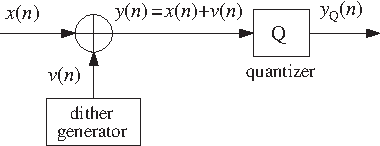
\includegraphics[width = 1\textwidth]{pic/ditherAdd.pdf}\\[0.2cm]
	\end{minipage}
	
	\subsection{Formen von Ditherrauschen}
		\begin{tabularx}{\textwidth}{|X|X|X|}
		 \hline
			\textbf{Gausssches Rauschen} & \textbf{Gleichverteiltes Rauschen} & \textbf{Dreieckverteiltes Rauschen}\\
		 \hline
			\begin{tikzpicture}[>=latex', scale=1.3]
				\def\si{0.5};
				\def\u{1.5};
				\draw[line width=0.75,->](-1.7,0)--(1.8,0)node[right]{\footnotesize$v$};
				\draw[line width=0.75,->](0,-0.1)--(0,1.9)node[right]{\footnotesize$p(v)$};
				\draw[smooth,samples=100,domain=-1.7:1.7, CadetRed, line width=1] plot (\x,{2/(sqrt(2*pi)*\si)*exp(-1/2*((\x)/\si)^2)});
				\draw[line width=0.75, black](0,0.1)--(0,-0.1) node [below] {\footnotesize$\mu=0$};
				\draw[line width=0.75, fill,white](0.3,0.95)--(0.6,0.95)--(0.6,1.1)--(0.3,1.1);

				\draw[line width=0.75, black,<->](0,0.85)--node [above, xshift=15pt , yshift=-2pt]{\footnotesize$\sigma_v = \frac{1}{2}Q$}(1.5-0.93,0.85);

				\draw[line width=0.75, black,<->](0,0.85)--node [above]{\footnotesize$ $}(1.5-2.07,0.85) ;
				\draw[line width=0.5](1.5,0.1)--(1.5,-0.1)node[below]{\footnotesize$\frac{3}{2} Q$};
				\draw[line width=0.5](-1.5,0.1)--(-1.5,-0.1)node[below]{\footnotesize$-\frac{3}{2} Q$};
			\end{tikzpicture}&
			\begin{tikzpicture}[>=latex', scale=1.3]
				\draw[->][line width=0.75](0,-0.3)--(0,1.2)node[right]{\footnotesize$p(v)$};
				\draw[->][line width=0.75](-1.7,0)--(1.8,0)node[below]{\footnotesize$v$};
				\draw[line width=1,CadetRed](-1.5,0)--(-1,0)--(-1,0.7)node[left]{\footnotesize$1/Q$}--(1,0.7)--(1,0)--(1.5,0);
				\draw[line width=0.5](-1,0.1)--(-1,-0.1)node[below]{\footnotesize -$Q/2$};
				\draw[line width=0.5](1,0.1)--(1,-0.1)node[below]{\footnotesize$Q/2$};
			\end{tikzpicture}&
			\begin{tikzpicture}[>=latex', scale=1.3]
				\draw[->][line width=0.75](0,-0.3)--(0,1.2)node[right]{\footnotesize$p(v)$};
				\draw[->][line width=0.75](-1.7,0)--(1.8,0)node[below]{\footnotesize$v$};
				\draw[line width=1,CadetRed](-1.7,0)--(-1.5,0)--(0,0.7)node[left, yshift=4pt]{\footnotesize$1/Q$}--(1.5,0)--(1.7,0);
				\draw[line width=0.5](-1.5,0.1)--(-1.5,-0.1)node[below]{\footnotesize -$Q$};
				\draw[line width=0.5](1.5,0.1)--(1.5,-0.1)node[below]{\footnotesize$Q$};
			\end{tikzpicture}\\
		 \hline&&\\[-0.3cm]
			$p(v) = \dfrac{\e^{-v^2/(2\,\sigma_v^2)}}{\sqrt{2\pi\sigma_v^2}}$&$p(v) = \begin{cases}\dfrac{1}{Q}, & -\frac{1}{2}Q\leq v\leq \frac{1}{2}Q\\0,& \text{sonst}\end{cases}$&$p(v) = \begin{cases}\dfrac{Q-|v|}{Q^2}, & -Q\leq v\leq Q\\0,& \text{sonst}\end{cases}$\\[0.65cm]
		 \hline&&\\[-0.3cm]
			$\sigma_v^2 = \frac{1}{4}Q^2$ & $\sigma_v^2 = \frac{1}{12}Q^2$&$\sigma_v^2 = \frac{1}{6}Q^2$\\[0.2cm]
		 \hline&&\\[-0.3cm]
			\fcolorbox{CadetRed}{white}{$\sigma_\varepsilon^2 = \frac{1}{12}Q^2 + \frac{1}{4}Q^2 = \frac{1}{3}Q^2$} &\fcolorbox{CadetRed}{white}{$\sigma_\varepsilon^2 = \frac{1}{12}Q^2 + \frac{1}{12}Q^2 = \frac{1}{6}Q^2$}&\fcolorbox{CadetRed}{white}{$\sigma_\varepsilon^2 = \frac{1}{12}Q^2 + \frac{1}{6}Q^2 = \frac{1}{4}Q^2$}\\[0.3cm]
		 \hline&&\\[-0.3cm]
			$4\times$ mehr Rauschen $(6\db)$ & $2\times$ mehr Rauschen $(3\db)$ & $3\times$ mehr Rauschen $(4.8\db)$\\[0.2cm]
		 \hline 
		\end{tabularx}\\

	\subsection{Subtractives Dither-Rauschen}
		\begin{minipage}{1\textwidth}
			Da das Dither-Rauschen selber erzeugt wurde kann es nach dem Quantisieren auch wieder abgezogen werden. Der Fehler reduziert sich dadurch wieder auf den Fehler des Quantisierungsrauschens.\\[0.2cm]
			\fcolorbox{CadetRed}{white}{$\varepsilon(n) = y_{out}(n)-x(n) = e(n)$}$\qquad$\fcolorbox{CadetRed}{white}{$\sigma_\varepsilon^2 = \frac{1}{12}Q^2$}
		\end{minipage}\\[0.5cm]
% 		\begin{minipage}{0.05\textwidth}$ $\end{minipage}
		\begin{minipage}{0.7\textwidth}
			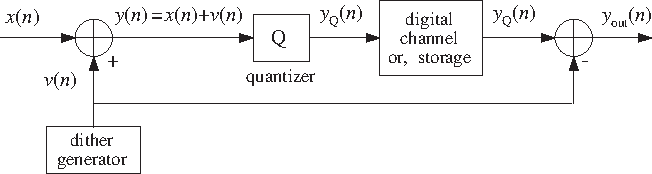
\includegraphics[width = \textwidth]{pic/ditherSub.pdf}\\[0.2cm]
		\end{minipage}



